\chapter{Results}
\label{sec:results}

We performs a variety of experiments to answer the following questions:  1) How good is our affordance model? 2) How well can \ours learn and improve in the real world? 3) How can the experience collected by \ours be distilled into a policy? 4) How can \ours be used for complex, soft object manipulation? We investigate the role of the affordance model and real-world fine-tuning in Table~\ref{tab:main} and Figure~\ref{fig:graph_main}. Then we perform a series of ablations in Table~\ref{tab:abl}.

\begin{table}[t]
    \centering
    \resizebox{\linewidth}{!}
    {%
        \begin{tabular}{lcccccccccccccccc}
        \toprule
        Method & \multicolumn{2}{c}{Pick cup} & \multicolumn{2}{c}{Pour cup} & \multicolumn{2}{c}{Open drawer} & \multicolumn{2}{c}{Pick spoon} & \multicolumn{2}{c}{Scoop Grape} & \multicolumn{2}{c}{Stir Spoon} & \\ 
        & train & test & train & test & train & test & train & test & train & test & train & test \\
        \midrule
        \
        \textbf{\texttt{Real-World Only}} & 0.0 & 0.1 & 0.2 & 0.1 & 0.1 & 0.0 & 0.7 & 0.3 & 0.0 & 0.0 & 0.3 & 0.0 \\ 
        \textbf{\texttt{Affordance Model Only}} & \multicolumn{2}{c}{0.1} & \multicolumn{2}{c}{0.4} & \multicolumn{2}{c}{\textbf{0.5}} & \multicolumn{2}{c}{0.5} & \multicolumn{2}{c}{0.0} & \multicolumn{2}{c}{0.3}\\ 
        
        \midrule
        \textbf{\texttt{\ours}} & \textbf{0.8} & \textbf{0.8} & \textbf{0.8} & \textbf{0.9} & \textbf{0.5} & \textbf{0.4} & \textbf{0.8} & \textbf{0.6} & \textbf{0.7} & \textbf{0.3} & \textbf{0.8} & \textbf{0.5}\\
        %%\textbf{\texttt{\ours First Iteration}} & 0.0 & 0.0 & 0.1 & 0.0 & 0.4 & 0.2 & 0.6 & 0.5 & 0.1 & 0.2 & 0.5 & 0.4\\ 
        \bottomrule
        \end{tabular}
    }
    \vspace{0.05in}
    \caption{We present the results of our method as well as compare them to other baselines: Real-world learning without internet priors used as guidance and the affordance model outputs without real-world learning.  Together, our method is able to better complete these tasks.}
    \label{tab:main}
\end{table}



\begin{figure}[t]
\centering
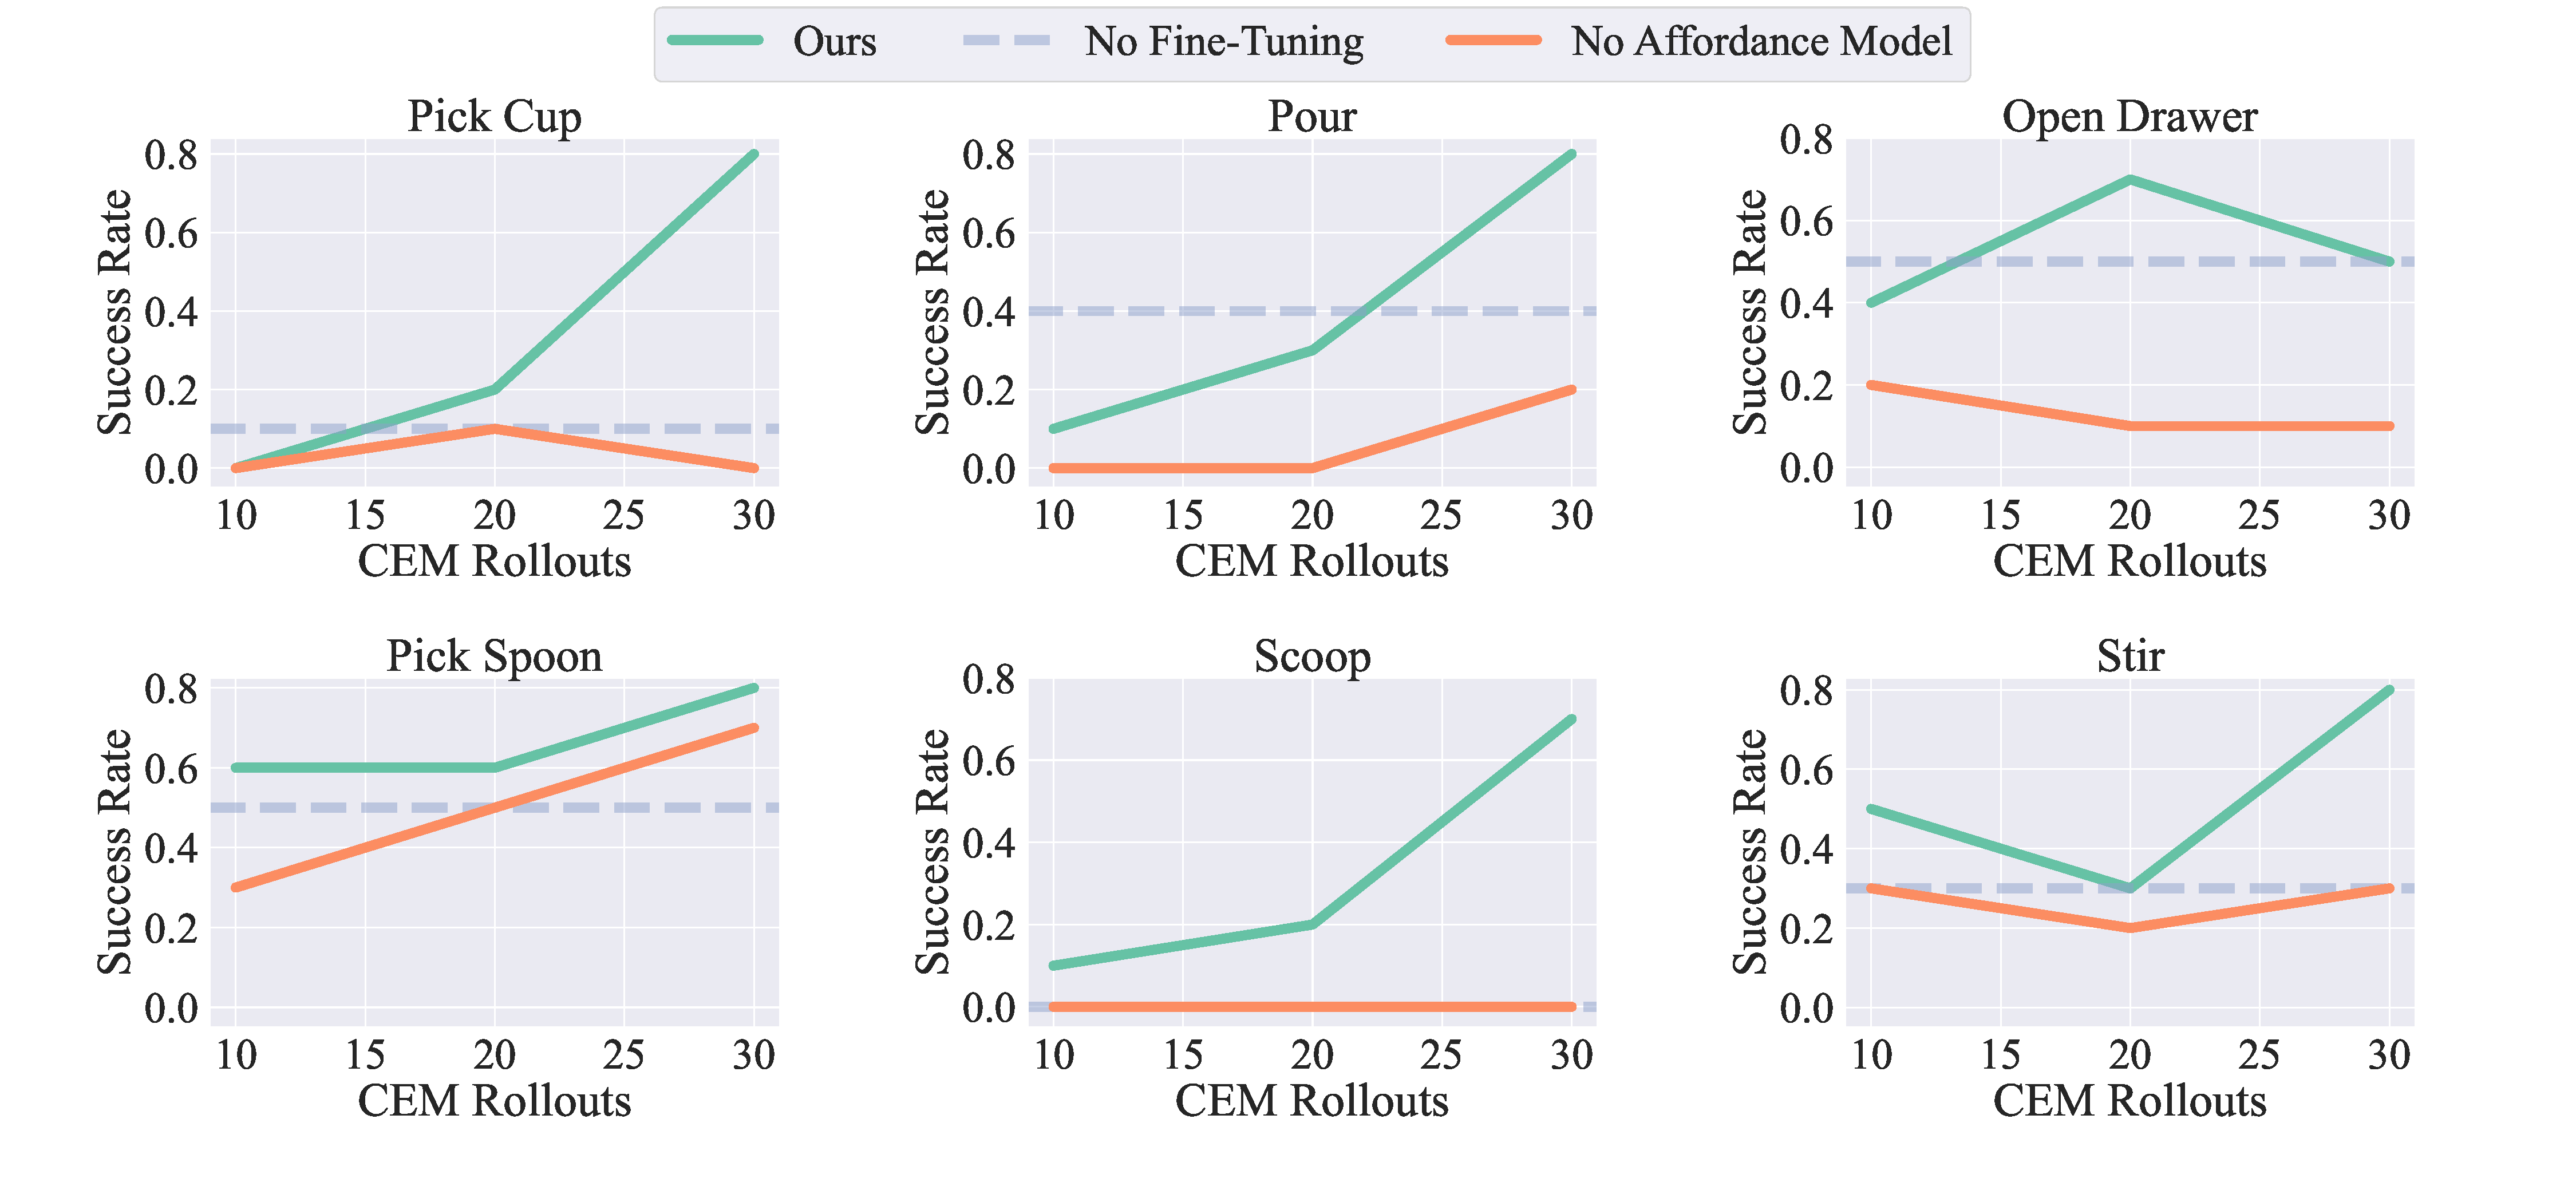
\includegraphics[width=\linewidth]{figs/graphs_main.pdf}
\vspace{-0.25in}
  \caption{\small Improvement results for 6 tasks: pick cup, pour, open drawer, pick spoon, scoop, and stir. We see a steady improvement in our method as more CEM episodes are collected.
}
 \label{fig:graph_main}
 \vspace{0.1in}
\end{figure}


\section{Effect of affordance prior} 
The human affordance model predicted three items: the contact location, the wrist grasp rotation, and and the hand joint pose. In the Real-World Only model, we use a few heuristics in place of each item in the affordance prior and proceed with fine-tuning. For contact location, we detect the object in the scene using a popular object detection model \cite{kirillov2023segment} and let the contact location prior be the center of the bounding box. For the wrist rotation, use a generic rotation with the pal of the hand facing downward. Finally, for the hand joint angles, we fix a half-closed hand as the grasp pose prior.  

With these heuristics, the robot has difficulty finding stable grasps consistently across a range of tasks. While the robot is able to navigate to the object, the main obstacle was finding the correct rotation angle for the hand. Hand rotation is very important for many tool manipulation tasks because it requires not only picking the tool but also grasping in a stable manner. While the soft hand shows decent success in grasping a spoon (where the grasp rotation from the heuristic is close to the correct grasp rotation) it is not able to perform well in tasks that require other wrist rotations.

It is possible that with more exploration the Real-World Only model would be able to catch up with \ours. However, we believe that these results indicate that the human affordance model reduces the number of fine-tuning episodes necessary in the real world.

\section{Zero-shot model execution} 
We explore the zero-shot performance of our prior with the Affordance Only model.  Without applying any online fine-tuning to our affordance model, we rollout the trajectory parameterized by the prior.  While our model performs decent on simpler tasks, the model struggles on tasks like stir and scoop that require strong, power grasps (shown in Table~\ref{tab:main}). In these tasks, the spoon collides with other objects, so fine-tuning the prior to hold the back of the spoon is important in maintaining a reliable grip throughout the post-grasp motion. Because \ours incorporates real-world experience with the prior, it is able to sample contact locations and grasp rotations that can better execute the task. 

One observation we found is that our zero-shot model sometimes performs better than the residual model trained on the first ten CEM iterations. This is due to \ours optimizing the grasp parameters only after ten iterations. Our first residual model learns only from random noise, explaining why our zero-shot performance can be stronger than \ours after few iterations of fine-tuning.


\begin{figure}[t]
\centering
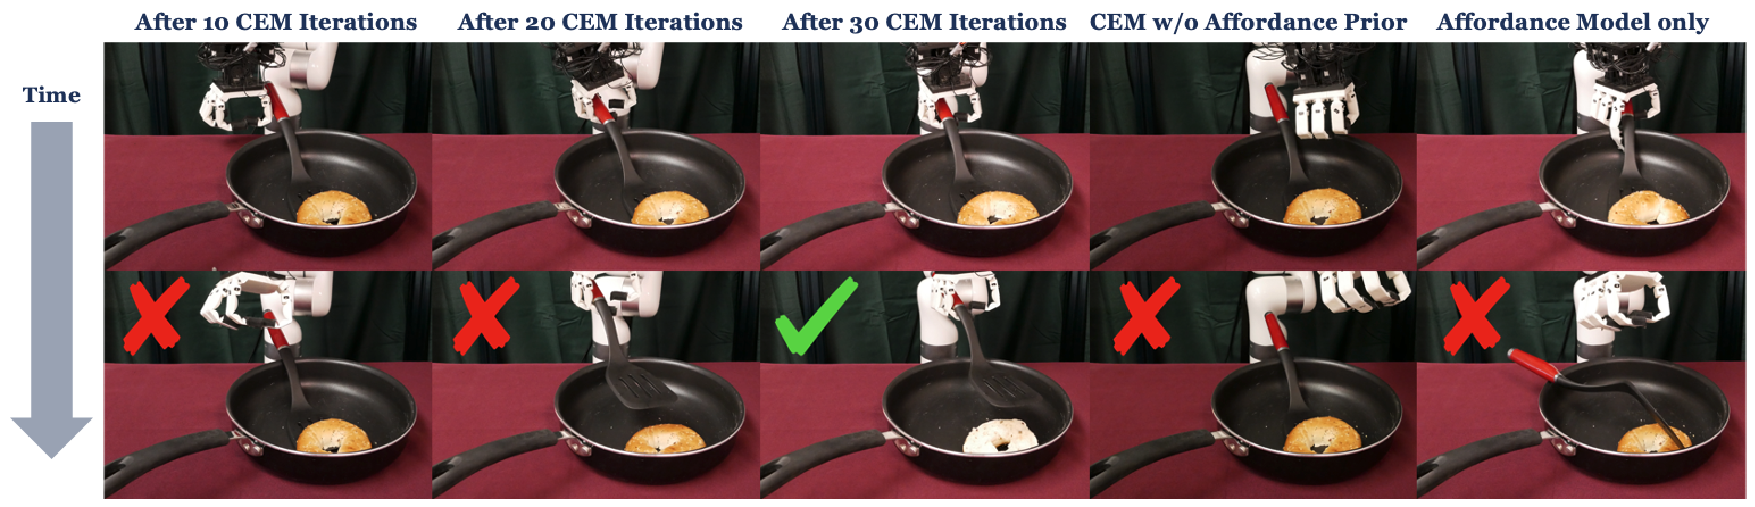
\includegraphics[width=\linewidth]{figs/qual_results.pdf}
\vspace{-0.2in}
  \caption{\small Qualitative results showing the finetuning procedure for \ours.  The model learns to hold the spatula and flip the bagel after 30 CEM iterations. }
 \label{fig:task_bagel}
 \vspace{-0.15in}
\end{figure}


\section{Human and automated rewards}
Our method queries the operator during the task reset process to assign a continuous score from $0$ to $1$ for the grasp.  Because the reset process requires a human-in-the-loop regardless, this adds little marginal cost for the operator.  But what if we would like these rewards to be calculated autonomously?  

We use the final image collected in the single post-grasp human demonstration from Section \ref{sec:method} as the goal image.  We define the reward to be the negative embedding distance between the final image of the rollout and the goal image with either an R3M \cite{r3m} or a ResNet \cite{resnet} encoder. The model learned from ranking trajectories with R3M reward is competitive with \ours in two of the three tasks we tested on, and performed better than the model that used Resnet18 rewards. Using a third-person camera could potentially improve the rankings because changes in the object will be more apparent. Nevertheless, these results indicate that using a visual reward model can potentially provide reasonable results compared to human rewards.

\begin{table}[t]
    \centering
    \resizebox{0.85\linewidth}{!}
    {%
        \begin{tabular}{lcccccc}
        \toprule
        Method & \multicolumn{2}{c}{Pour Cup} & \multicolumn{2}{c}{Open Drawer} & \multicolumn{2}{c}{Pick Spoon}  \\ 
         &train & test & train & test & train & test\\
        \midrule
        \multicolumn{2}{l}{\textit{Reward Function:}}\vspace{0.0em}\\
        \textbf{\texttt{R3M Reward}} & 0.0 & 0.0 & 0.4 & \textbf{0.5} & 0.5 & 0.4\\ 
        \textbf{\texttt{Resnet18 Imagenet Reward}} & 0.1 & 0.2 & 0.3 & 0.1 & 0.4 & 0.2\\ 
        \midrule
        \multicolumn{2}{l}{\textit{Policy Ablation:}}\vspace{0.0em}\\
        \textbf{\texttt{\ours w/ MLP}} & 0.0 & 0.0 & 0.5 & 0.0 & 0.6 & 0.5\\ 
        \textbf{\texttt{\ours w/ Transformer}} & 0.4 & 0.5 & \textbf{0.6} & 0.1 & 0.4 & 0.5\\  
        \textbf{\texttt{\ours w/ Direct Parameter est.}} & 0.1 & 0.1 & 0.1 & 0.0 & 0.3 & 0.0\\ 
        \midrule
        \textbf{\texttt{\ours }} & \textbf{0.8} & \textbf{0.9} & 0.5 & 0.4 & \textbf{0.8} & \textbf{0.6} \\ 
        \bottomrule
        \end{tabular}
    }
    \vspace{0.05in}
    \caption{Ablations for (1) reward function type, (2) model architecture, and (3) parameter estimation approach.}
    \label{tab:abl}
\end{table}


\section{Model Architecture} We investigate different models and training architectures for the policy trained on the rollouts (Table~\ref{tab:abl}). When we replace the conditional VAE with an MLP that predicts residuals, the model has difficulty learning the grasp rotation to effectively pour a cup. This may be because VAEs can compress multi-modal data more effectively (which is useful for our case as our data includes location, rotation, and joint angles).

Our transformer ablation is an offline method similar to \cite{chen2021decisiontransformer} where in addition to the image and affordance model outputs, we condition on the reward outputs and train a transformer to predict the residual. At test time the maximum reward is queried and the output is used in the rollout. We hypothesize that the reduced performance is because the transformer is a data-hungry architecture. The model may need more real-world data, which can be expensive to collect.

Finally, we train a VAE to directly estimate $\xi$ instead of the residual. This model was unable to effectively distill the information from the affordance prior with neither the diversity of data nor training time allotted. As a result, it often makes predictions that are far from the correct grasp pose. 


\begin{figure}[t]
\vspace{-0.2in}
\begin{center}
    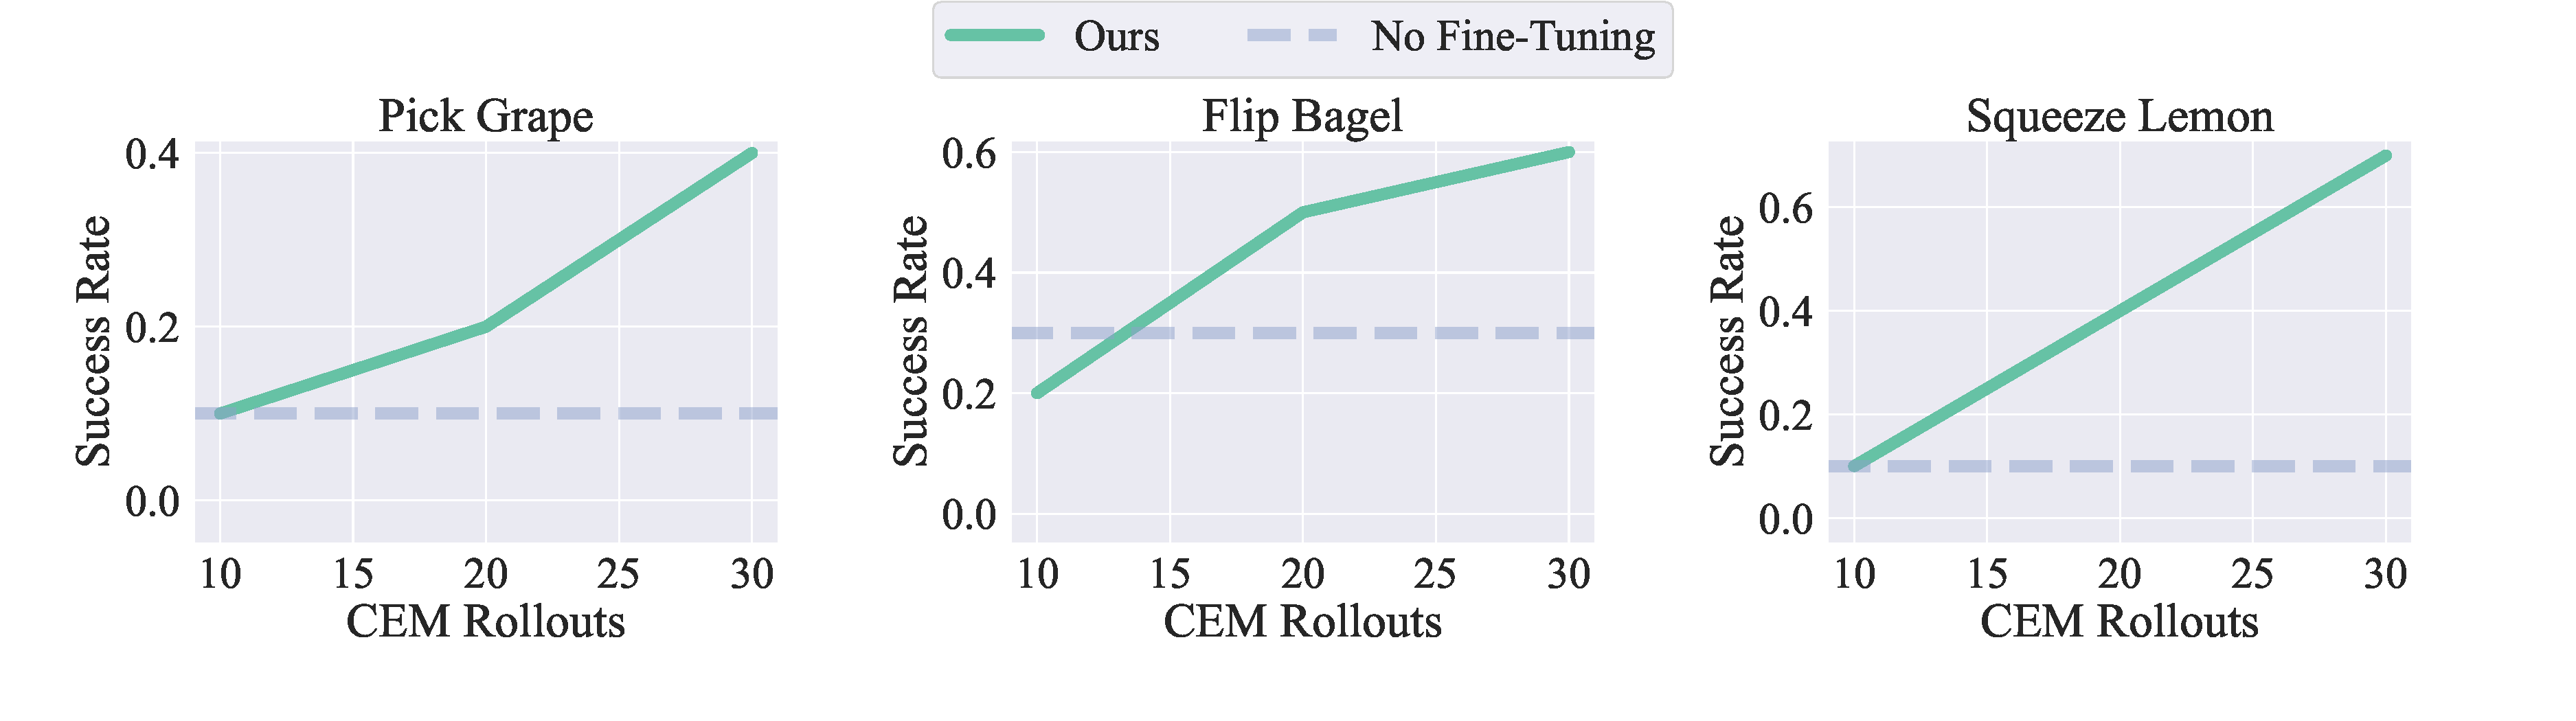
\includegraphics[width=\linewidth]{figs/graphs_difficult.pdf}
\end{center}
\vspace{-0.1in}
  \caption{\footnotesize We evaluate \ours on three additional difficult manipulation tasks. }
 \label{fig:graph_difficult}
 \vspace{-0.15in}
\end{figure}


\section{Performance on complex tasks and soft objects} 
We investigate the performance of \ours on more challenging tasks, which involve grasping or manipulating food. Tasks involving soft objects cannot be simulated accurately, so sim2real methods may have difficulty performing these tasks in the real world. Our method does not have that challenge in this setting and \ours is able to perform reasonably well after on these tasks.

Of the three tasks, our method has the most difficulty with the Pick Grape task. This is because grapes are small and require the fingers to curl fully to maintain a stable grasp. A limitation of our hand is that the range of MCP joint does not allow the fingertips to touch its palm, and as a result it has difficulty in consistently picking small objects.
